\section{Projektmanagement Planung}
Für die Organisation des Projektes wurde der webbasierte Hosting-Dienst
GitHub verwendet. Auf einem über GitHub erstellten Verzeichnis (Repository
genannt) werden alle relevanten Daten fürs Projekt zentral gespeichert und
sind so für alle Teammitglieder über das Internet ständig zugänglich. Die
Verwaltung der Daten erfolgt über ein gleichnamiges Programm oder direkt
über das verteilte Versionsverwaltungssystem Git. Werden Änderungen an
einer Datei vorgenommen, wird diese vom Programm erkannt und kann vom
Benutzer anschliessend commited (Bestätigung zur Übernahme der Änderung)
werden. Arbeiten zwei Teammitglieder gleichzeitig an der selben Datei
entsteht ein Konflikt, welcher in einem Merge-Prozess (Zusammenführen)
aufgelöst wird. Diese Konflikte lassen sich grösstenteils durch eine gute
Organisation und Arbeitsteilung vermeiden.

\begin{figure}[h!]
	\centering
	\includegraphics[scale=1]{../../fig/pm/repository.pdf}
	\caption{Grundstruktur der Organisation auf GitHub}
	\label{fig:gh-org}
\end{figure}

Mittels GitHub können sogenannte \emph{Issues} verwaltet werden. Diese
\emph{Issues} beschreiben jeweils eine konkrete Aufgabe. Diese können
einem Teammitglied zugewiesen werden, besitzen einen Status (offen,
erledigt) und werden zeitlich terminiert in dem sie einem
\emph{Meilenstein} zugewiesen werden. Diese \emph{Issues} ermöglichen
es so, die Aufgaben einfach und effektiv zu verteilen.

Die Aufgabenstellung dieses Projektes beinhaltete die Abgabe von 3
Berichten über den Verlauf des Semesters hinweg. Mittels Github wurde
für jede Abgabe jeweils ein \emph{Meilenstein} erstellt, welcher die
zu erledigenden Aufgaben bzw. \emph{Issues} für die Berichte
zusammenfasst. So ist sich jeder Nutzer bewusst, was er bis zur
Abgabe zu tun hat.

\subsection{Realisierung und Auswertung des Projektmanagement}
Wie im vorhergehenden Abschnitt erläutert, basiert das gesamte
Projektmanagement auf der aktiven Teilnahme aller Teammitglieder.
Die Systematik dieses Prozesses ist im Abschnitt 
\ref{sec:issue-management} erläutert. Dieser wird rückblickend
analysiert im Abschnitt \ref{sec:issue-analysis} mittels der Daten,
welche durch Git und GitHub zur Verfügung gestellt werden.
Anschliessend auf die Analyse ist ein Fazit welches Massnahmen zur
Optimierung des Arbeitspaketmanagements formuliert für die
Realisierungsphase des Projekts (PREN2).

\subsubsection{Arbeitspaketverwaltung}\label{sec:issue-management}
Die für den jeweiligen Meilenstein notwendigen Arbeitspakete werden im
Plenum definiert und als \emph{Issues} formuliert auf dem entsprechenden
\emph{Repository}. Im Anschluss wird zusammen bewertet und definiert,
welches Teammitglied die jeweilige Aufgabe optimal erfüllen kann.

\begin{figure}[h!]
	\centering
	\includegraphics[scale=1]{../../fig/pm/issue_01.pdf}
	\caption{Strategie der Arbeitspaketverwaltung}
	\label{fig:pm-issue-01}
\end{figure}

Nach der Formulierung und Zuteilung der Arbeitspakete wird anschliessend
nochmals kontrolliert, welches Teammitglied welche Aufgaben zugeteilt
bekommen hat. Hierfür bietet das Webinterface von GitHub eine
Filterfunktion an, mit welcher sich offene Arbeitspakete nach Benutzer
(\emph{assignee}) filtern lassen. Diese werden nochmals betrachtet und
es wird im Plenum entschieden, ob die jeweiligen Zuteilungen optimal
ausgelegt sind. So wird beispielsweise festgestellt, dass einem
Teammitglied zu viele Aufgaben zugeteilt sind. Wird dies bereits zu
diesem Zeitpunkt deutlich, so können einzelne Aufgaben um geteilt werden
um eine unausgeglichene Belastung der Teammitglieder zu verhindern.

Die erstellten und zugeteilten Arbeitspakete werden dann individuell
abgearbeitet und können als erledigt (\emph{closed}) markiert werden.
Der relative Stand des zugehörigen Meilensteins wird prozentual
berechnet aufgrund des Verhältnisses von offenen und erledigten
Arbeitspaketen. Dies ist insbesondere für den Projektleiter ein
Indikator für den Projektfortschritt.

\subsubsection{Analyse}\label{sec:issue-analysis}
Die Auswertung der Arbeitspaketverwaltung basiert auf den Daten, welche
durch die \emph{Commits} numerisch analysierbar und von GitHub zur
Verfügung gestellt sind. Für diese Auswertung gilt die Annahme, dass
alle Commits jeweils gleich gewichtet sind. Aus den zur Verfügung
stehenden Daten lassen sich drei Kriterien beurteilen:

\begin{itemize}
	\item Arbeitszeiten \hfill{} (\textit{wann wird gearbeitet})
	\item Kontinuität \hfill{} (\textit{wie kontinuierlich wird gearbeitet})
	\item Aufteilung \hfill{} (\textit{wie ist die Arbeitsaufteilung})
\end{itemize}

Die Arbeitszeiten werden mittels der \emph{punch card} bewertet, welche
in der Abbildung \ref{fig:gh-punchcard} dargestellt ist. Diese gibt die
relative Anzahl der \emph{commits} zum Wochentag und Tageszeit wieder.

\begin{figure}[h!]
	\centering
	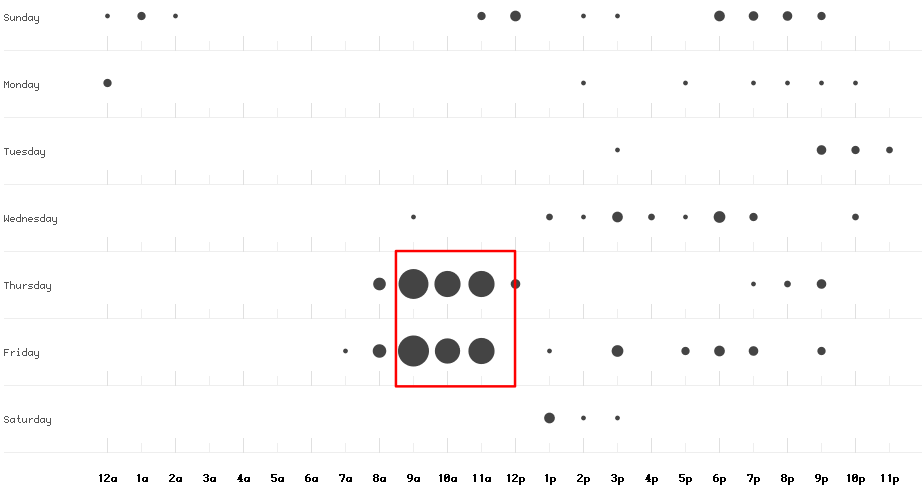
\includegraphics[width=0.85\textwidth]{../../fig/pm/gh-punchcard_marked.pdf}
	\caption{Punch card des ``doku'' Repository von ``accefa''
		(rot markiert die Blockzeiten des Moduls).}
	\label{fig:gh-punchcard}
\end{figure}

Diese zeigt deutlich, dass zu den vorgegebenen Blockzeiten des Moduls
die meisten \emph{commits} erfolgen. Diese Auffälligkeit hat verschiedene
Gründe. Zum einen ist die Arbeit mit den beschriebenen Tools für die
Mehrheit des Teams neu und ungewohnt. Dies erfordert des öfteren das
gemeinsame angehen gewisser Tasks, welche anschliessend in der Regel zu
einem \emph{commit} führen. Ein weiterer Grund, welcher zu dieser
Ansammlung von \emph{commits} führt, ist, dass die Bearbeitung der
zugeteilten \emph{issues} im Plenum besprochen und korrigiert wurde.

Die Auswertung der Kontinuität erfolgt mit dem Graphen der summierten
\emph{contributions} für den jeweiligen Tag über das gesamte
\emph{repository}. Dieser Graph ist in der Abbildung 
\ref{fig:gh-contributions-ov} dargestellt.

\begin{figure}[h!]
	\centering
	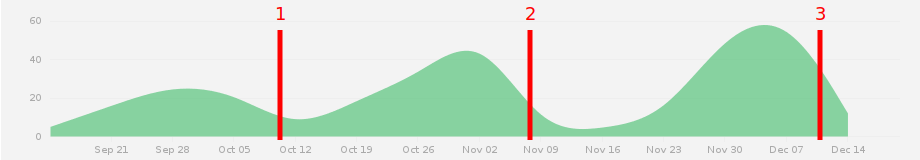
\includegraphics[width=1\textwidth]{../../fig/pm/gh-contributions-ov_marked.pdf}
	\caption{\emph{Contributions}-Verlauf des ``doku'' Repository
		von ``accefa'' (rot markiert die Meilensteine).}
	\label{fig:gh-contributions-ov}
\end{figure}

Dieser Graph zeigt eine markante Welligkeit auf, wobei die lokalen Extrema
kurz vor den Terminen der Meilensteine liegen. Dies deutet darauf hin, dass
die Arbeitsplanung gut organisiert ist und die Arbeitspakete deutlich vor
dem jeweiligen Meilenstein erledigt sind. Die Amplituden der Wellen
scheinen mit jedem Meilenstein zuzunehmen in einen linearen Zusammenhang,
während die Änderungsrate innerhalb einer Bearbeitungsperiode deutlich zunimmt.
Diese Beobachtung ist plausibel, da die Änderungsrate mit der Zunahme der
Dokumentation wächst.

Die Beobachtungen aus dem \emph{contributions}-Grpahen für das
\emph{Repository} sind in gleicher Weise bei allen Teammitglieder zu erkennen,
wie in der Abbildung \ref{fig:gh-contributions-team} dargestellt. Die einzelnen
Grpahen unterscheiden sich in der jeweiligen Ausprägung der Extremalstellen,
Teilen aber die Periodizität des allgemeinen Graphen. Dies ist gegeben durch
die relative Darstellung der Graphen, welche für jeden Benutzer einzeln
ausgewertet werden und somit keine absolute Aussage zulassen. Dies ist auch
deutlich ausgeweisen durch die \emph{commits}, \emph{additions} ($++$) und
\emph{deletions} ($--$).

\begin{figure}[h!]
	\centering
	\includegraphics[width=1\textwidth]{../../fig/pm/gh-contributions-team.png}
	\caption{\emph{Contributions}-Graphen der einzelnen Teammitglieder
		von \lstinline{accefa/doku}}
	\label{fig:gh-contributions-team}
\end{figure}

\subsubsection{Massnahmen zur Optimierung}\label{sec:issue-optize}
Die Analyse des Projektmanagement hinsichtlich der Arbeitspakete zeigt zwei
wesentliche Erkenntnisse auf. Zum einen sammeln sich Arbeiten zu den
gemeinsamen Projektzeiten an (siehe Abbildung \ref{fig:gh-punchcard}).
Dies deutet darauf hin, dass abseits der Blockzeiten, also während der
individuellen Bearbeitungszeit, nicht so intensiv gearbeitet wird oder
gearbeitet werden kann. Zum andern gibt es eine Diskontinuität von der
Arbeitsintensität, wobei das obere Extrema kurz vor den Meilensteinen liegt
(siehe Abbildung \ref{fig:gh-contributions-ov}).
Dies deutet darauf hin, dass viele Arbeitspakete erst vor den zugehörigen
Meilensteinen erledigt werden. Aus diesen Beobachtungen lassen sich
folgende Ziele für eine Optimierung des Projektmanagement formulieren.

\begin{enumerate}
	\item Die Arbeitspakete sollen kontinuierlicher abgearbeitet werden.
	\item Die Arbeitspakete sollen vermehrt ausserhalb der gemeinsamen
		Modulzeiten bearbeitet werden.
\end{enumerate}

\noindent
Um diese Ziele zu erreichen, sind entsprechende Massnahmen notwendig.
Mögliche Massnahmen, welche dann in der Realisierungsphase anzuwenden sind,
könnten die folgenden sein.

\begin{enumerate}
	\item Die erstellten Arbeitspakete sollen feiner ausgelegt werden.
		Dies ermöglicht eine schnellere Abarbeitung und reduziert
		die Besprechungsdauer bzw. das Review als auch die
		Nachbearbeitungszeit.
	\item Zu den offiziellen Meilensteinen sollen vorangehende
		Meilensteine angelegt werden. Sämtliche Arbeitspakete sollen
		diesen vorangehenden Meilensteinen zugewiesen werden.
		Dies verschafft einen zeitlichen Puffer für die Reviews als
		auch die Nachbearbeitung.
	\item Bei Unsicherheiten bezüglich eines zugewiesenen Arbeitspakets
		soll dieses nicht bis zur nächsten Sitzung aufgeschoben werden,
		sondern wird einfach einem anderen Teammitglied mit einem
		entsprechenden Kommentar zugewiesen. Dies reduziert die
		Latenzen und maximiert die Dynamik der Organisation.
\end{enumerate}

Die letzte Massnahme verändert die Systematik der Arbeitspaketverwaltung,
welche somit zu einer Anpassung der Prozessdarstellung führt, wie in der
Abbildung \ref{fig:pm-issue-02} dargestellt.

\begin{figure}[h!]
	\centering
	\includegraphics[scale=1]{../../fig/pm/issue_02.pdf}
	\caption{Verbesserte Arbeitspaketverwaltung zur Dynamikoptimierung}
	\label{fig:pm-issue-02}
\end{figure}


\subsection{Kostenübersicht}
Für unseres Projekt hatten wir ein Budget von 600.00 CHF. Die Kosten
wurden in einer Tabelle verwaltet um den Überblick zu wahren. Die
Schätzung für die Kosten wurden in der Kolonne Budget eingetragen. Die
Schätzung des Budget basiert auf Recherchen im Internet und sind jeweils
mit den maximal Kosten budgetiert. Aus dies ist anzunehmen, dass eher
weniger gebraucht wird, als budgetiert.

\begin{figure}[h!]
	\center
	\includegraphics[width=0.8\textwidth]{../../fig/Kostenuebersicht.jpg}
	\caption{Kostenübersicht}
	\label{fig:Kostenuebersicht}
\end{figure}

Das gesamt Budget des PREN-Projekts liegt bei 600.00 CHF. Bisher rechnen
wir damit, dass 500.00 CHF für ein erfolgreiches umsetzen reichen sollten.
Die restlichen 100.00 CHF dienen als gute Reserve für das Korrigieren von
Fehlentscheidungen. Im PREN 1 durfte 200.00 CHF ausgegeben werden, davon
wurde 85.40 CHF gebraucht. 

\subsection{Projekteam}

\begin{tabularx}{\columnwidth}{XX}
	
	\textbf{Adriano Valsangiacomo} \newline
	Maschinentechnik \newline
	\href{mailto:adriano.valsangiacomo@stud.hslu.ch}{adriano.valsangiacomo@stud.hslu.ch} \newline
	
	&  
	
	\textbf{Ervin Mazlagi\'c} \newline
	Elektrotechnik \newline
	\href{mailto:ervin.mazlagic@stud.hslu.ch}{ervin.mazlagic@stud.hslu.ch} \newline 
	
	\\ 
	
	\textbf{Christian Spycher} \newline
    Maschinentechnik \newline
    \href{mailto:christian.spycher@stud.hslu.ch}{christian.spycher@stud.hslu.ch} \newline 
     
    
    & 
    
    \textbf{Fabian Wüthrich} \newline
    Informatik \newline
    \href{mailto:fabian.wuethrich.01@stud.hslu.ch}{fabian.wuethrich.01@stud.hslu.ch} \newline 
    
    \\ 
	
	\textbf{Christian Schürch} \newline
	Maschinentechnik \newline
	\href{mailto:christian.schuerch@stud.hslu.ch}{christian.schuerch@stud.hslu.ch} \newline 
	
	& 
	 
	\textbf{Alexander Suter} \newline
	Informatik \newline
	\href{mailto:alexander.suter@stud.hslu.ch}{alexander.suter@stud.hslu.ch} \newline 
	
	\\ 
\end{tabularx} 


\subsection{Organigramm}
Die Hierarchie des Projektteams ist im Organigramm in Abbildung \ref{fig:organigramm} dargestellt.

\begin{figure}[h!]
	\centering
	\begin{tikzpicture}
	\node [draw](projektleiter) {
		\begin{tabular}{c}
		Projektleiter \\
		Adriano \\
		Valsangiacomo
		\end{tabular} 
	};
	
	\node [draw, below left =1cm and 2cm of  projektleiter] (informatik) {Informatik} edge [<-] (projektleiter);
	\node [draw, below =1cm of  projektleiter] (elektrotechnik) {Elektrotechnik} edge [<-] (projektleiter);
	\node [draw, below right =1cm and 2cm of  projektleiter] (mechanik) {Mechanik} edge [<-] (projektleiter);
	
	\node [draw, below left  = of  informatik] (fabianwuethrich) {
			\begin{tabular}{c}
			Fabian \\
			Wüthrich
			\end{tabular}
		} edge [<-] (informatik);
	\node [draw, below right = of  informatik] (alexsuter) {
			\begin{tabular}{c}
			Alexander \\
			Suter
			\end{tabular} 
		} edge [<-] (informatik);
	
	\node [draw, below =3cm of  elektrotechnik] (ervinmazlagic) {
			\begin{tabular}{c}
			Ervin \\
			Mazlagi\'c
			\end{tabular}
		} edge [<-] (elektrotechnik);
	
	\node [draw, below left = of  mechanik] (christianspycher) {
		\begin{tabular}{c}
		Christian \\
		Spycher
		\end{tabular} 
		} edge [<-] (mechanik);
	\node [draw, below = of  mechanik] (christianschuerch) {
		\begin{tabular}{c}
		Christian \\
		Schürch
		\end{tabular}} edge [<-] (mechanik);
	\node [draw, below right = of  mechanik] (adrianovalsangiacomo) {
				\begin{tabular}{c}
				Adriano \\
				Valsangiacomo
				\end{tabular}  
		  } edge [<-] (mechanik);
	\end{tikzpicture}
	\caption{Organigramm}
	\label{fig:organigramm}
\end{figure}


\begin{landscape}
\subsection{Risikoanalyse}
\begin{table}[h!]
    \small
    \centering
    \begin{tabular}{p{0.08\textwidth} c p{0.15\textwidth} p{0.4\textwidth} p{0.15\textwidth} p{0.1\textwidth} p{0.2\textwidth}}
		& Nr. & Risiko & Ursache & Wahrscheinlichkeit & Auswirkung & Massnahmen \\
        \hline \hline
        & & & & & & \\
        \rowcolor{yellow} Personelle Faktoren 
            & 1 
            & Falscher Projektleiter 
            & Falsche Vorstellungen vom Projekt 
            & Vorstellbar 
            & gering 
            & Erfolg darf nicht vom Projektleiter abhängen \\ 
        \rowcolor{yellow}
	        & 2 
            & Zwei Mitglieder einer Studienrichtung fallen aus 
            & Krankheit, Studienabbruch 
            & Unwahrscheinlich 
            & Katastrophal 
            & externe Hilfe holen \\
        \rowcolor{green}
            & 3 
            & Betreuender Dozent fällt aus 
            & Krankheit, beschäftigt mit anderen Projekten 
            & vorstellbar 
            & unwesentlich 
            & \\
        \rowcolor{yellow}
            & 4	
            & Team verstreitet sich	
            & unterschiedliche Ansichten, falsche Arbeitsplanung, unterschiedlicher Arbeitseinsatz, fehlende Verbindlichkit	
            & Vorstellbar 
            & Katastrophal 
            & Arbeit genau Planen, offene Kommunikation, Verbindlichkeiten schafen \\
        \rowcolor{yellow}
            & 5	
            & Ungenügende Kommunikation 
            & ungenügende Planung, fehlende Interdisziplinarität, schlechte Stimmung im Team 
            & Vorstellbar 
            & Katastrophal 
            & offen und oft Kommunizieren, Rückmeldungen geben \\
        \rowcolor{yellow}
            & 6	
            & 
            & 
            & 
            & 
            & \\
        \rowcolor{yellow} Zeitliche Faktoren 
            & 7 
            & Zu optimistische Ressourcenplanung 
            & hohe Belastung durch das Studium, zu komplexe Lösungsvarianten 
            & Vorstellbar 
            & Kritisch 
            & realistisch Planen, komplexität verringern \\
	    \rowcolor{yellow}
            & 8 
            & mangelnde Produktivität 
            & Überforderung, schlechte Planung, desinteresse, fehlende Zeitplanung 
            & Unwahrscheinlich 
            & Kritisch 
            & gute Planung, Verbindlichkeiten schafen \\
        \rowcolor{yellow}
	        & 9 
            & Ungenügende Zeitkontrolle 
            & unklare Zeitplanung 
            & Vorstellbar 
            & Kritisch 
            & Reflektion der Arbeiten, Meilensteine festlegen \\
        \rowcolor{yellow}
	        & 10 
            & Unklare Zeitplanung 
            & Zeitplanung unverbindlich oder nicht vorhanden 
            & Vorstellbar 
            & Kritisch 
            & Realistisch Planen, verbindliche Zeitplanung \\
        \rowcolor{yellow}
	        & 11 
            & 
            & 
            & 
            & 
            & \\
        \rowcolor{red} Technische Faktoren 
            & 12 
            & Unerwarteter Datenverlust 
            & Diebstall, Unachtsamkeit, schlechte Organisation 
            & Gelegentlich 
            & Katastrophal 
            & Arbeit auf mehreren Platformen speichern \\
        \rowcolor{green} 
            & 13 
            & Fehlende Fachkentnisse 
            & zu hohe Ansprüche 
            & Unwahrscheinlich 
            & Geringfügig 
            & externe Hilfe hohlen, komplexität verringern \\
        \rowcolor{yellow}
	        & 14 
            & Nicht zu resultierender Lösungsvorschlag 
            & zu hohe Ansprüche, fehlende Prototypen, schlechte Planung 
            & Unwahrscheinlich 
            & Kritisch 
            & Prototypen erstellen, komplexität verringern \\
        \rowcolor{yellow} 
            & 15 
            & 
            & 
            & 
            & 
            & \\
	\end{tabular}
\end{table}
\end{landscape}


\subsubsection{Risiko-Bewertungsschema}
\begin{table}[h!]
	\renewcommand{\arraystretch}{1.5}
	\centering
	\begin{tabular}{r || c c c c}
		häufig 		
			& \cellcolor{red} 
			& \cellcolor{red}
			& \cellcolor{red}
			& \cellcolor{red} \\
		wahrscheinlich		
			& \cellcolor{yellow} 
			& \cellcolor{yellow} 
			& \cellcolor{red}
			& \cellcolor{red} \\
		gelegentlich		
			& \cellcolor{yellow}
			& \cellcolor{yellow}
			& \cellcolor{yellow}
			& \cellcolor{red} \\
		vorstellbar		
			& \cellcolor{green}
			& \cellcolor{yellow}
			& \cellcolor{yellow}
			& \cellcolor{yellow} \\
		unwahrscheinlich	
			& \cellcolor{green}
			& \cellcolor{green}
			& \cellcolor{yellow}
			& \cellcolor{yellow} \\
		unvorstellbar		
			& \cellcolor{green}
			& \cellcolor{green}
			& \cellcolor{green}
			& \cellcolor{green} \\
		\hline
		& unwesentlich & geringfügig & kritisch & katastrophal
	\end{tabular}
\end{table}

